\documentclass{sig-alternate-05-2015}
\usepackage{times,amsmath,amsfonts,amssymb,epstopdf,xspace}
\usepackage{graphicx}
\usepackage{hyperref}
\usepackage[usenames]{color}


\newcommand{\red}[1]{{\textcolor{red}{#1}}}

\pdfminorversion=7


%Journals
\newcommand{\mnras}{MNRAS}
\newcommand{\jcap}{JCAP}
\newcommand{\physrep}{Phys.~Rep.}   % Physics Reports
\newcommand{\apjs}{ApJS}

% Latex tricks
\newcommand{\oh}[1]{\mbox{$ {\mathcal O}( #1 ) $}}
\newcommand{\eqn}[1] {(\ref{eqn:#1})}


% Some acronyms
\newcommand{\swift}{{\sc swift}\xspace}
\newcommand{\qs}{{\sc QuickShed}\xspace}

% Webpage
\newcommand{\web}{\url{www.swiftsim.com}}


%#####################################################################################################

\begin{document}

%Conference
\conferenceinfo{PASC '16}{June 8--10, 2016, Lausanne, Switzerland}

\title{{\ttlit SWIFT}: Using task-based parallelism, fully asynchronous
communication, and graph partition-based domain decomposition for
strong scaling on more than 100\,000 cores.}
% \title{{\ttlit SWIFT}: A task-based hybrid-parallel strongly scalable code for
%   particle-based cosmological simulations}

\numberofauthors{6}
  
\author{
\alignauthor
       Matthieu~Schaller\\
       \affaddr{Institute for Computational Cosmology (ICC)}\\
       \affaddr{Department of Physics}\\
       \affaddr{Durham University}\\
       \affaddr{Durham DH1 3LE, UK}\\
       \email{\footnotesize \url{matthieu.schaller@durham.ac.uk}}
\alignauthor
       Pedro~Gonnet\\
       \affaddr{School of Engineering and Computing Sciences}\\
       \affaddr{Durham University}\\
       \affaddr{Durham DH1 3LE, UK}\\
\alignauthor
       Aidan~B.~G.~Chalk\\
       \affaddr{School of Engineering and Computing Sciences}\\
       \affaddr{Durham University}\\
       \affaddr{Durham DH1 3LE, UK}\\
\and
\alignauthor
       Peter~W.~Draper\\
       \affaddr{Institute for Computational Cosmology (ICC)}\\
       \affaddr{Department of Physics}\\
       \affaddr{Durham University}\\
       \affaddr{Durham DH1 3LE, UK}\\
       %% \alignauthor
       %% Tom Theuns\\
       %% \affaddr{Institute for Computational Cosmology}\\
       %% \affaddr{Department of Physics}\\
       %% \affaddr{Durham University}\\
       %% \affaddr{Durham DH1 3LE, UK}      
}


\date{\today}

\maketitle

%#####################################################################################################

\begin{abstract}
  We present a new open-source cosmological code, called \swift, designed to
  solve the equations hydrodynamics using a particle-based approach (Smooth
  Particle Hydrodynamics) on hybrid shared / distributed clusters and the
  task-based library \qs, the parallelisation backbone of \swift. The code
  relies on three main aspects to make efficient use of current and future
  architectures:

  \begin{itemize}
    
    \item \textbf{Task-based parallelism} to exploit shared-memory
      parallelism. This provides fine-grained load balancing enabling
      strong scaling, combined with mixing communication and
      computation, both on each node with multiple cores.

    \item \textbf{Asynchronous hybrid shared/distributed memory
      parallelism}, using the task-based schemes. Parts of the
      computation are scheduled only once the asynchronous transfers
      of the required data have completed. Communication latencies are
      thus hidden by computation, providing for strong scaling across
      thousands of multi-core nodes.

    \item \textbf{Graph-based domain decomposition}, which uses
      information from the task graph to decompose the simulation
      domain such that the work, as opposed to just the data, as in
      other space-filling curve schemes, is equally distributed
      amongst all nodes.

  \end{itemize}

  %% These three main aspects alongside improved cache-efficient
  %% algorithms for neighbour finding allow the code to be 40x faster on
  %% the same architecture than the standard code Gadget-2 widely used by
  %% researchers.

  These algorithms do not rely on a specific architecture nor on detailed
  micro-level details.  As a result, our code present excellent \emph{strong}
  scaling on a variety of architectures, ranging from x86 Tier-2 systems to the
  largest Tier-0 machines currently available. It displays, for instance, a
  \emph{strong} scaling parallel efficiency of more than 60\% when going from
  512 to 131072 cores on a BlueGene architecture. Similar results are obtained
  on standard clusters of x86 CPUs.
  
  %% The task-based library, \qs, used as the backbone of the code is
  %% itself also freely available and can be used in a wide variety of
  %% other numerical problems.
  
\end{abstract}


\keywords{Physics; Cosmology; Fluid dynamics; Smooth Particle Hydrodynamics;
  Task-based parallelism; Asynchronous data transfer; Extreme scaling}

%#####################################################################################################


\section{Introduction}

For the past decade, due to the physical limitations
on the speed of individual processor cores, instead of
getting {\em faster}, computers are getting {\em more parallel}.
Systems containing up to 64 general-purpose cores are becoming
commonplace, and the number of cores can be expected to continue
growing exponentially, e.g.~following Moore's law, much in the
same way processor speeds were up until a few years ago.

As a consequence, in order to get any faster, computer programs
need to rely on better exploiting this massive parallelism, i.e.~
they need to exhibit {\em strong scaling}, the ability to run
roughly $N$ times faster when executed on $N$ times as many processors.
Without strong scaling, massive parallelism can still be used to
tackle ever {\em larger} problems, but not fixed-size problems
{\em faster}.

Although this switch from growth in speed to growth in parallelism
has been anticipated and observed for quite some time, very little
has changed in terms of how we design and implement parallel
computations, e.g.~branch-and-bound synchronous parallelism using
OpenMP\cite{ref:Dagum1998} and MPI\cite{ref:Snir1998}, and domain
decompositions based on space-filling curves \cite{warren1993parallel}.

The design and implementation of \swift \cite{gonnet2013swift,%
theuns2015swift,gonnet2015efficient}, a large-scale cosmological
simulation code built from scratch, provided the perfect
opportunity to test some newer approaches, i.e.~task-based parallelism,
fully asynchronous communication, and graph partition-based
domain decompositions.
This paper describes the results obtained with these parallelisation
techniques.


%#####################################################################################################

\section{Particle-based hydrodynamics}

Smoothed Particle Hydrodynamics \cite{Gingold1977,Price2012} (SPH) uses
particles to represent fluids.  Each particle $p_i$ has a position $\mathbf
x_i$, velocity $\mathbf v_i$, internal energy $u_i$, mass $m_i$, and a smoothing
length $h_i$.  The particles are used to interpolate any quantity $Q$ at any
point in space as a weighted sum over the particles:
%
\begin{equation}
    Q(\mathbf r) = \sum_i m_i \frac{Q_i}{\rho_i} W( \|\mathbf r - \mathbf r_i\| , h )
    \label{eqn:interp}
\end{equation}
%
where $Q_i$ is the quantity at the $i$th particle, $h$ is the {\em smoothing
  length}, i.e.~the radius of the sphere within which data will be considered
for the interpolation, and $W(r,h)$ is the {\em smoothing kernel} or {\em
  smoothing function}.  Several different forms for $W(r,h)$ exist, each with
their own specific benefits and drawbacks.

The particle density $\rho_i$ used in \eqn{interp} is itself computed similarly:
%
\begin{equation}
    \rho_i = \sum_{j,~r_{ij} < h_i} m_j W(r_{ij},h_i)
    \label{eqn:rho}
\end{equation}
%
where $r_{ij} = \|\mathbf{r_i}-\mathbf{r_j}\|$ is the Euclidean distance between
particles $p_i$ and $p_j$.  In compressible simulations, the smoothing length
$h_i$ of each particle is chosen such that the number of neighbours with which
it interacts is kept more or less constant, and can result in smoothing lengths
spanning several orders of magnitudes within the same simulation.

Once the densities $\rho_i$ have been computed, the time derivatives of the
velocity and internal energy, which require $\rho_i$, are
computed as followed:
%
\begin{eqnarray}
    \frac{dv_i}{dt} & = & -\sum_{j,~r_{ij} < \hat{h}_{ij}} m_j \left[
        \frac{P_i}{\Omega_i\rho_i^2}\nabla_rW(r_{ij},h_i) +
        \frac{P_j}{\Omega_j\rho_j^2}\nabla_rW(r_{ij},h_j) \right], \label{eqn:dvdt} \\ 
    \frac{du_i}{dt} & = & \frac{P_i}{\Omega_i\rho_i^2} \sum_{j,~r_{ij} < h_i} m_j(\mathbf v_i - \mathbf v_j) \cdot \nabla_rW(r_{ij},h_i), \label{eqn:dudt}
\end{eqnarray}
%
where $\hat{h}_{ij} = \max\{h_i,h_j\}$, and the particle pressure $P_i=\rho_i
u_i (\gamma-1)$ and correction term $\Omega_i=1 +
\frac{h_i}{3\rho_i}\frac{\partial \rho}{\partial h}$ are computed on the fly.

The computations in \eqn{rho}, \eqn{dvdt}, and \eqn{dudt} involve finding all
pairs of particles within range of each other.  Any particle $p_j$ is {\em
  within range} of a particle $p_i$ if the distance between $p_i$ and $p_j$ is
smaller or equal to the smoothing distance $h_i$ of $p_i$, e.g.~as is done in
\eqn{rho}.  Note that since particle smoothing lengths may vary between
particles, this association is not symmetric, i.e. $p_j$ may be in range of
$p_i$, but $p_i$ not in range of $p_j$.  If $r_{ij} < \max\{h_i,h_j\}$, as is
required in \eqn{dvdt}, then particles $p_i$ and $p_j$ are within range {\em of
each other}.

The computation thus proceeds in two distinct stages that are evaluated
separately:
\begin{enumerate}
    \item {\em Density} computation: For each particle $p_i$,
        loop over all particles $p_j$ within range of $p_i$ and evaluate
        \eqn{rho}.
    \item {\em Force} computation: For each particle $p_i$,
        loop over all particles $p_j$
        within range of each other and evaluate \eqn{dvdt} and \eqn{dudt}.
\end{enumerate}

Finding the interacting neighbours for each particle constitutes
the bulk of the computation.
Many codes, e.g. in Astrophysics simulations \cite{Gingold1977},
the above-mentioned approaches cease to work efficiently.
rely on spatial {\em trees}
for neighbour finding \cite{Gingold1977,Hernquist1989,Springel2005,Wadsley2004},
i.e.~$k$-d trees \cite{Bentley1975} or octrees \cite{Meagher1982}
are used to decompose the simulation space.
In Astrophysics in particular, spatial trees are also a somewhat natural
choice as they are used to compute long-range gravitational interactions
via a Barnes-Hut \cite{Barnes1986} or Fast Multipole
\cite{Carrier1988} method. 
The particle interactions are then computed by traversing the list of
particles and searching for their neighbours in the tree.

Although such tree traversals are trivial to parallelize, they
have several disadvantages, e.g.~with regards to computational
efficiency, cache efficiency, and exploiting symmetries in the
computation (see \cite{gonnet2015efficient} for a more detailed
analysis).


%#####################################################################################################

\section{Parallelisation strategy}

\subsection{Task-based parallelism}

Task-based parallelism is a shared-memory parallel programming
paradigm in which a computation is broken-down in to a set of
{\em tasks} which can be executed  concurrently.
In order to ensure that the tasks are executed in the right
order, e.g.~that data needed by one task is only used once it
has been produced by another task, and that no two tasks
update the same data at the same time, {\em dependencies} between
tasks are specified and strictly enforced by a task scheduler.
Computations described in this way then parallelize trivially:
each processor repeatedly grabs a task for which all dependencies
have been satisfied and executes it until there are no tasks left.

The main advantages of using a task-based approach are
%
\begin{itemize}
    \item The order in which the tasks are processed is completely
        dynamic and adapts automatically to load imbalances.
    \item If the dependencies and conflicts are specified correctly,
        there is no need for expensive explicit locking, synchronisation,
        or atomic operations to deal with most concurrency problems.
    \item Each task has exclusive access to the data it is working on,
        thus improving cache locality and efficiency.
        If each task operates exclusively on a restricted part of the
        problem data, this can lead to high cache locality and efficiency.
\end{itemize}
%
Task-based parallelism is not a particularly new concept and therefore
several implementations thereof exist, e.g.~Cilk \cite{ref:Blumofe1995},
QUARK \cite{ref:QUARK}, StarPU \cite{ref:Augonnet2011},
SMP~Superscalar \cite{ref:SMPSuperscalar}, OpenMP~3.0 \cite{ref:Duran2009},
and Intel's TBB \cite{ref:Reinders2007}.

For convenience, and to make experimenting with different scheduling
techniques easier, we chose to implement our own task scheduler
in \swift, which has since been back-ported as the general-purpose
\qs task scheduler \cite{gonnet2013quicksched}.
This also allowed us to extend the scheduler with the concept of
{\em conflicts}: two tasks conflict if they cannot be executed
concurrently, e.g.~because the access some common resource or memory
location, yet the order in which they are executed is irrelevant.

Despite its advantages, and the variety of implementations,
task-based parallelism is rarely used in
practice (notable exceptions include the PLASMA project
\cite{ref:Agullo2009} which uses QUARK/StarPU, and the {\tt deal.II} project
\cite{ref:Bangerth2007} which uses Intel's TBB).
The main problem is that to effectively use task-based parallelism,
most computations need to be completely redesigned to fit the paradigm,
which is usually not an option for existing large and complex codebases.

Since we were re-implementing \swift from scratch, this was not an issue.
The tree-based neighbour-finding described above was replaced with a more
task-friendly approach as described in \cite{gonnet2015efficient}.
Particle interactions are computed within, and between pairs, of
hierarchical {\em cells} containing one or more particles.
The dependencies between the tasks are set following
equations \eqn{rho}, \eqn{dvdt}, and \eqn{dudt}, i.e. such that for any cell,
all the tasks computing the particle densities therein must have
completed before the particle forces can be computed, and all the
force computations must have completed before the particle velocities
may be updated.

Due to the cache-friendly nature of the task-based computations, 
and their ability to exploit symmetries in the particle interactions,
the task-based approach is already more efficient than the tree-based
neighbour search on a single core, and scales efficiently to all
cores of a shared-memory machine \cite{gonnet2015efficient}.


\subsection{Task-based domain decomposition}

Given a task-based description of a computation, partitioning it over
a fixed number of nodes is relatively straight-forward: we create
a {\em cell hypergraph} in which:
\begin{itemize}
  \item Each {\em node} represents a single cell of particles, and
  \item Each {\em edge} represents a single task, connecting the
    cells used by that task.
\end{itemize}
Since in the particular case of \swift each task references at most
two cells, the cell hypergraph is just a regular {\em cell graph}.

Any partition of the cell graph represents a partition of the
computation, i.e.~the nodes belonging to each partition each belong
to a computational {\em rank} (to use the MPI terminology), and the
data belonging to each cell resides on the partition/rank to which
it has been assigned.
Any task spanning cells that belong to the same partition needs only
to be evaluated on that rank/partition, and tasks spanning more than
one partition need to be evaluated on both ranks/partitions.

If we then weight each edge with the computational cost associated with
each task, then finding a {\em good} partitioning reduces to finding a
partition of the cell graph such that:
\begin{itemize}
  \item The weight of the edges within each partition is more or less
    equal, and
  \item The weight of the edges spanning two or more partitions is
    minimal.
\end{itemize}
\noindent where the first criteria provides good {\em load-balancing},
i.e.~each partition/rank should involve the same amount of work, and
the second criteria reduces the {\em partition cost}, i.e.~the amount
of duplicated work between partitions/ranks.

Computing such a partition is a standard graph problem and several
software libraries which provide good solutions\footnote{Computing
the optimal partition for more than two nodes is considered NP-hard.},
e.g.~METIS \cite{ref:Karypis1998} and Zoltan \cite{devine2002zoltan},
exist.

Note that this approach does not explicitly consider any geometric
constraints, or strive to partition the {\em amount} of data equitably.
The only criteria is the computational cost of each partition, for
which the task decomposition provides a convenient model.
We are therefore partitioning the {\em computation}, as opposed
to just the {\em data}.

Note also that the proposed partitioning scheme takes neither the
task hierarchy, nor the size of the data that needs to be exchanged
between partitions/ranks into account.
This approach is therefore only reasonable in situations in which
the task hierarchy is wider than flat, i.e.~the length of the critical
path in the task graph is much smaller than the sum of all tasks,
and in which communication latencies are negligible.


\subsection{Asynchronous communications}


%#####################################################################################################

\section{Scaling tests}

In this section we present some strong scaling tests of the \swift code on different
architectures for a representative cosmology problem.

\subsection{Simulation setup}

The initial distribution of particles used in our tests is extracted and
resampled from low-redshift outputs of the EAGLE project \cite{Schaye2015}, a
large suite of state-of-the-art cosmological simulations. By selecting outputs
at late times, we constructed a simulation setup which is representative of the
most expensive part of these simulations, i.e. when the particles are
highly-clustered and not uniformly distributed anymore. This distribution of
particles is shown on Fig.~\ref{fig:ICs} and periodic boundary conditions are
used. In order to fit our simulation setup into the limited memory of some of
the systems tested, we have randomly down-sampled the particle count of the
output to $800^3=5.12\times10^8$, $600^3=2.16\times10^8$ and
$300^3=2.7\times10^7$ particles respectively. We then run the \swift code for
100 time-steps and average the wall clock time of these time-steps after having
removed the first and last ones, where i/o occurs.

\begin{figure}
\centering
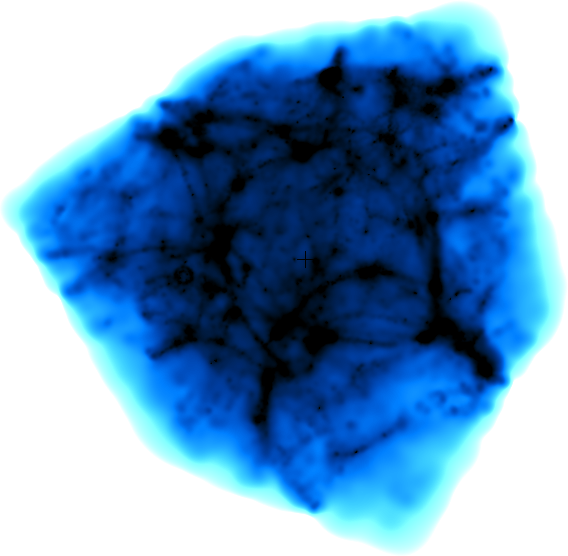
\includegraphics[width=\columnwidth]{Figures/cosmoVolume}
\caption{The initial density field computed from the initial particle
  distribution used for our tests. The density $\rho_i$ of the particles spans 8
  orders of magnitude, requiring smoothing lengths $h_i$ changing by a factor of
  almost $1000$ across the simulation volume. \label{fig:ICs}}
\end{figure}  


\subsection{x86 architecture: Cosma-5}

For our first test, we ran \swift on the cosma-5 DiRAC2 Data Centric
System\footnote{\url{icc.dur.ac.uk/index.php?content=Computing/Cosma}} located
at the University of Durham. The system consists of 420 nodes with 2 Intel Sandy
Bridge-EP Xeon
E5-2670\footnote{\url{http://ark.intel.com/products/64595/Intel-Xeon-Processor-E5-2670-20M-Cache-2_60-GHz-8_00-GTs-Intel-QPI}}
clocked at $2.6~\rm{GHz}$ with each $128~\rm{GByte}$ of RAM. The nodes are
connected using a Mellanox FDR10 Infiniband 2:1 blocking configuration.

The code was compiled with the Intel compiler version \textsc{2016.0.1} and
linked to the Intel MPI library version \textsc{5.1.2.150} and metis library
version \textsc{5.1.0}.



\subsection{x86 architecture: SuperMUC}

For our next test, we ran \swift on the SuperMUC x86 phase 1 thin
nodes \footnote{\url{https://www.lrz.de/services/compute/supermuc/systemdescription/}}
located at the Leibniz Supercomputing Centre in Garching near Munich. This
system is made of 9,216 nodes with 2 Intel Sandy Bridge-EP Xeon E5-2680
8C\footnote{\url{http://ark.intel.com/products/64583/Intel-Xeon-Processor-E5-2680-(20M-Cache-2_70-GHz-8_00-GTs-Intel-QPI)}}
at $2.7~\rm{GHz}$ with each $32~\rm{GByte}$ of RAM. The nodes are split in 18
``islands'' of 512 nodes within which communications are handled via an
Infiniband FDR10 non-blocking Tree. Islands are then connected using a 4:1
Pruned Tree.

The code was compiled with the Intel compiler version \textsc{2015.5.223} and
linked to the Intel MPI library version \textsc{5.1.2.150} and metis library
version \textsc{5.0.2}.

The simulation setup with $800^3$ particles was run on that system using 16 to
2048 nodes (4 islands) and the results of this strong scaling test are shown on
Fig.~\ref{fig:superMUC}. For this test, we used one MPI rank per node and 16
threads per node (i.e. one thread per physical core).

\begin{figure*}[t]
\centering
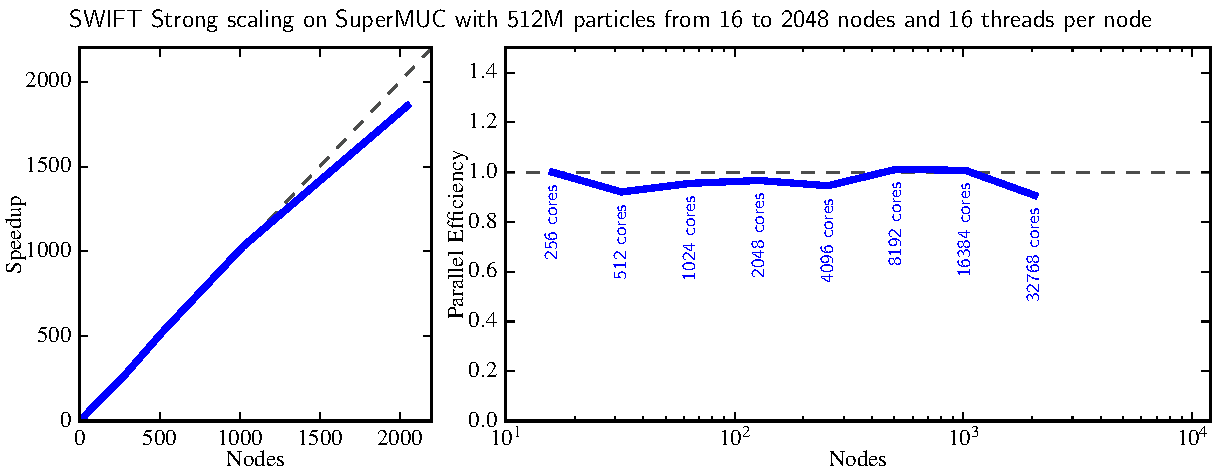
\includegraphics[width=\textwidth]{Figures/scalingSuperMUC}
\caption{Strong scaling test on the SuperMUC phase 1 machine (see text
  for hardware description). \textit{Left panel:} Code
  Speed-up. \textit{Right panel:} Corresponding parallel efficiency.
  Using 16 threads per node (no use of hyper-threading) with one MPI rank
  per node, an almost perfect parallel efficiency is achieved when
  increasing the node count from 16 (512 cores) to 2,048 (32,768
  cores).
  \label{fig:superMUC}}
\end{figure*}


\subsection{BlueGene architecture: JUQUEEN}

For our last set of tests, we ran \swift on the JUQUEEN IBM BlueGene/Q
system\footnote{\url{http://www.fz-juelich.de/ias/jsc/EN/Expertise/Supercomputers/JUQUEEN/Configuration/Configuration_node.html}}
located at the J\"ulich Supercomputing Centre. This system is made of 28,672
nodes consisting of an IBM PowerPC A2 processor running at $1.6~\rm{GHz}$ with
each $16~\rm{GByte}$ of RAM. Of notable interest is the presence of two floating
units per compute core. The system is composed of 28 racks containing each 1,024
nodes. The network uses a 5D torus to link all the racks.

The code was compiled with the IBM XL compiler version \textsc{30.73.0.13} and
linked to the corresponding MPI library and metis library
version \textsc{4.0.2}.

The simulation setup with $600^3$ particles was first run on that system using
512 nodes with one MPI rank per node and variable number of threads per
node. The results of this test are shown on Fig.~\ref{fig:JUQUEEN1}.

We later repeated the test, this time varying the number of nodes from 32 to
8192 (8 racks).  For this test, we used one MPI rank per node and 32 threads per
node (i.e. two threads per physical core). The results of this strong scaling
test are shown on Fig.~\ref{fig:JUQUEEN2}.


\begin{figure}
\centering
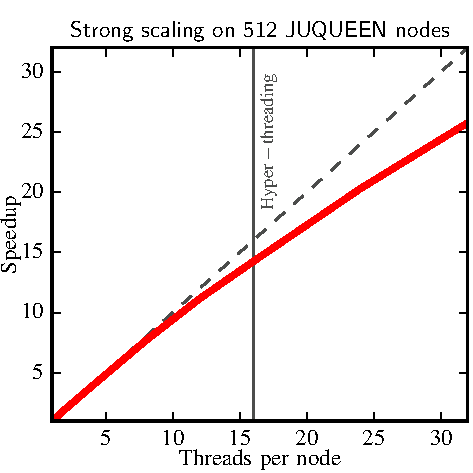
\includegraphics[width=\columnwidth]{Figures/scalingInNode}
\caption{Strong scaling test of the hybrid component of the code. The
  same calculation is performed on 512 node of the JUQUEEN BlueGene
  machine (see text for hardware description) with varying number of
  threads per node. The number of MPI ranks per node is kept fixed to
  one. The code displays excellent scaling even when all the cores and
  hardware multithreads are in use. \label{fig:JUQUEEN1}}
\end{figure}  



\begin{figure*}[t]
\centering
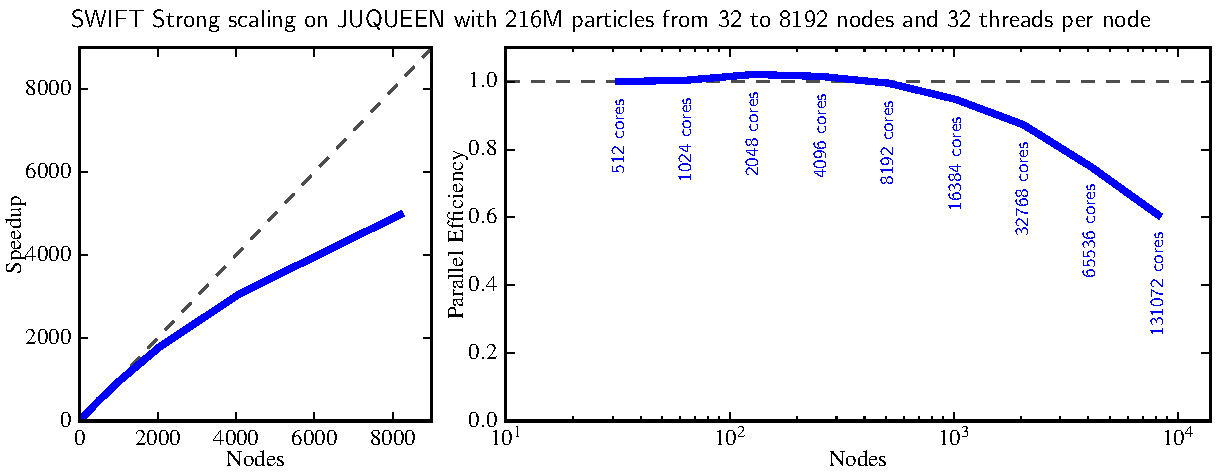
\includegraphics[width=\textwidth]{Figures/scalingBlueGene}
\caption{Strong scaling test on the JUQUEEN BlueGene machine (see text
  for hardware description). \textit{Left panel:} Code
  Speed-up. \textit{Right panel:} Corresponding parallel efficiency.
  Using 32 threads per node (2 per physical core) with one MPI rank
  per node, a parallel efficiency of more than $60\%$ is achieved when
  increasing the node count from 32 (512 cores) to 8,192 (131,072
  cores). On 8,192 nodes there are fewer than 27,000 particles per
  node and only a few hundred tasks, making the whole problem
  extremely hard to load-balance effectively.
  \label{fig:JUQUEEN2}}
\end{figure*}





%#####################################################################################################

\section{Conclusions}

When running on the SuperMUC machine with 32 nodes (512 cores), each MPI rank
contains approximately $1.6\times10^7$ particles in $2.5\times10^5$
cells. \swift will generate around $58,000$ point-to-point asynchronous MPI
communications (a pair of \texttt{Isend} and \texttt{Irecv}) per node every
time-step. 


%#####################################################################################################

\section{Acknowledgements}
This work would not have been possible without Lydia Heck's help and
expertise. We thank Heinrich Bockhorst and Stephen Blair-Chappell from
{\sc intel} as well as Dirk Brommel from the J\"ulich Computing Centre
and Nikolay J. Hammer from the Leibniz Rechnenzentrum for their help
at various stages of this project.\\ This work used the DiRAC Data
Centric system at Durham University, operated by the Institute for
Computational Cosmology on behalf of the STFC DiRAC HPC Facility
(\url{www.dirac.ac.uk}). This equipment was funded by BIS National
E-infrastructure capital grant ST/K00042X/1, STFC capital grant
ST/H008519/1, and STFC DiRAC Operations grant ST/K003267/1 and Durham
University. DiRAC is part of the National E-Infrastructure. This work
was supported by the Science and Technology Facilities Council
ST/F001166/1 and the European Research Council under the European
Union's ERC Grant agreements 267291 ``Cosmiway'', and by {\sc intel}
through establishment of the ICC as an {\sc intel} parallel computing
centre (IPCC).

\nocite{*}
\bibliographystyle{abbrv}
\bibliography{biblio}


\end{document}
